\documentclass{article}
\usepackage{mhchem}
\usepackage{chemfig}
\usepackage[german]{babel}
\usepackage{amsthm}
\usepackage{xifthen}
\usepackage{graphicx}


% from https://gist.github.com/malloc47/5298181 
\newcommand{\oneline}[1]{
  \newdimen{\namewidth}
  \setlength{\namewidth}{\widthof{#1}}
  \ifthenelse{\lengthtest{\namewidth < \textwidth}}
  {#1}% do nothing if shorter than text width
  {\resizebox{\textwidth}{!}{#1}}% scale down
}

\graphicspath{ {./images/} }

\title{Kunststoffe}
\author{Phillip Zazzetta}
\begin{document}

\newtheorem*{definition}{Definition}
\maketitle

\section*{Kunststoffe}
\begin{definition}
    Kunststoffe: synthetische organische Werkstoffe, die aus Polymeren bestehen
\end{definition}
\begin{definition}
    Monomer: kleinste Einheit eines Makromoleküls
\end{definition} 
\begin{definition}
    Polymer: Makromoleküle, die aus aneinandergereihten Makromolekülen bestehen
\end{definition}

\begin{minipage}[t]{0.3\textwidth}
    \subsection*{Thermoplasten}
    \subsubsection*{Eigenschaften}
    \begin{itemize}
        \item werden beim Erwärmen leicht und formbar
        \item behalten beim Abkühlen ihre Form
        \item verhalten sich wie Gemische (keine definierten Schmelzpunkte)
    \end{itemize} 

    \subsubsection*{Struktur}
    \textbf{amorph}\\
    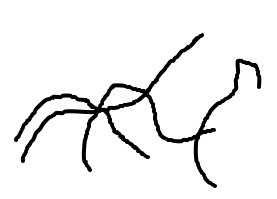
\includegraphics[width=\textwidth]{amorph}
    \textbf{teilkristallin}\\
    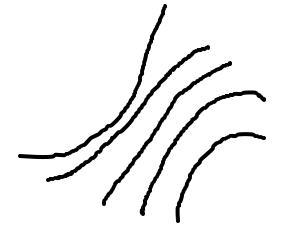
\includegraphics[width=\textwidth]{teilkristallin}

    \subsubsection*{stabilisierende Kräfte}
    einzelne Makromoleküle werden durch zwischenmolekulare Wechselwirkungen(
        WW. zw. temp. Dip., WW. zw. perm. Dip)
    stabilisiert

    \subsubsection*{Beispiele}
    PE (Polyethen)
    \newline $\rightarrow$ Flaschen, Folien
    \newline PVC (Polyvinylchlorid)
    \newline \oneline{$\rightarrow$ Schallplattten, Fußböden}
    \newline PET, PP, PS, ...
  \end{minipage}\hfill
  \begin{minipage}[t]{0.3\textwidth}
    \subsection*{Duroplasten}
    \subsubsection*{Eigenschaften}
    \begin{itemize}
        \item hart, später nicht mehr verformbar
        \item zersetzen sich beim Erhitzen
        \item unlöslich
    \end{itemize}

    \subsubsection*{Struktur}
    \textbf{verknüpft}
    \includegraphics[width=\textwidth]{verknüpft}

    \subsubsection*{stabilisierende Kräfte}
    Makromoleküle sind engmaschig durch Elektronenpaarbindungen verknüpft

    \subsubsection*{Beispiele}
    \oneline{Melamin- bzw Phenolharze}
    \newline $\rightarrow$ Lacke, Isolationsteile, Verbundswerkstoffe

  \end{minipage}\hfill
  \begin{minipage}[t]{0.3\textwidth}
    \subsection*{Elastomere}
    \subsubsection*{Eigenschaften}
    \begin{itemize}
        \item verändern durch mech. Belastung ihre Form, kehren aber wieder in den Ausgangszustand zurück
        \item zersetzen sich beim Erhitzen
        \item werden beim Abkühlen hart und spröde
    \end{itemize}

    \subsubsection*{Struktur}
    \textbf{teilverknüpft}
    \includegraphics[width=\textwidth]{teilverknüpft}

    \subsubsection*{stabilisierende Kräfte}
    Makromoleküle sind weitmaschig durch Elektronenpaarbindungen verknüpft

    \subsubsection*{Beispiele}
    Silikon
    \newline \oneline{$\rightarrow$ Dichtunge, Backformen}
    \newline Synthesekautschuk
    \newline \oneline{$\rightarrow$ Reifen, Gummibänder}
\end{minipage}

\section*{Der Lange Weg zum Kunststoff}
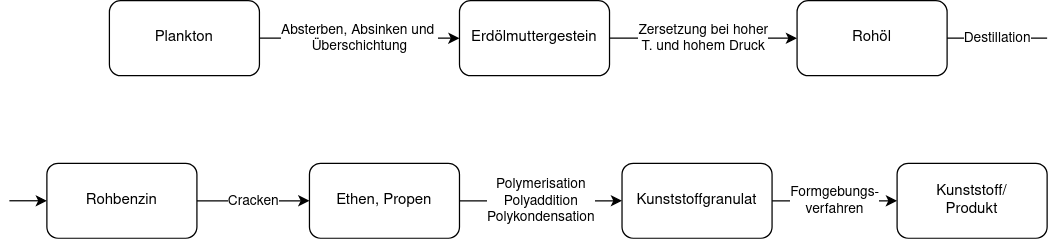
\includegraphics[width=\textwidth, keepaspectratio]{Der_lange_Weg_zum_Kunststoff}

\section*{Eigenschaften von Kunststoffen}
\begin{table}[h]
    \begin{tabular}{llllll}
    Probe & \begin{tabular}[c]{@{}l@{}}Brennbarkeit \\ in Flamme\end{tabular} & außerhalb & \begin{tabular}[c]{@{}l@{}}Verformbarkeit \\ kalt\end{tabular} & warm & Dichte in g/cm³ \\
    PE    & +                                                                 & +         & +                                                              & ++   & 0.9             \\
    PVC   & + (rußt)                                                          & -         & +                                                              & ++   & 1.44            \\
    PF    & 0                                                                 & -         & --                                                             & --   & 1.41            \\
    PS    & +                                                                 & -         & -                                                              & +    & 1.04            \\
    PA    & + (rußt)                                                          & -         & +                                                              & ++   & 1.17            \\
    PMMA  & ++                                                                & +         & 0                                                              & +    & 1.18            \\
    UP    & 0 (rußt)                                                          & -         & --                                                             & --   & 1.95           
    \end{tabular}
    \end{table}

\section*{Synthese von Kuststoffen}
\subsection*{Polymerisation}
\subsubsection*{Beispiel PVC (Polyvinylchlorid)}
\schemestart
\chemname{\chemfig{C(-[3]H)(-[5]H)(=C(-[1]H)(-[7]Cl))}}{Vinylchlorid (1-Chlorethen)}
\arrow{->[Initiator]}
\chemleft{[}
\chemfig{-[0,0.5]C(-[:90]H)(-[:-90]H)(-C(-[:90]H)(-[:-90]H)(-[:0,0.5]))}
\chemright{]}
\schemestop
\end{document}